\label{sec:hessian}
%\rnote{Title of this section is a bit long and don't have a real focus. We might consider break it into multiple sections? One possibility is that we talk about the decomposition, then talk about properties of $xx^\T$ (both zero-mean and non-zero-mean case) and briefly talk about properties of $M$ (mostly empirical); in the next section we can then use this decomposition to justify (a) Hessian overlap; (b) low rank structure of the top eigenvectors; (c) rank C-1 Hessian}
The fact that layer-wise Hessian for a single sample can be decomposed into Kronecker product of two components naturally leads to the following informal conjecture:
\begin{conjecture}[Decoupling Conjecture] The layer-wise Hessian can be approximated by a Kronecker product of the expectation of its two components, that is
\begin{equation}
    \HessL(\vw^{(p)}) = \E[\mM\otimes \vx\vx^\T] \approx \E[\mM] \otimes \E[\vx\vx^\T].
    \label{eqn:decouple}
\end{equation}
More specifically, we conjecture that 
%\begin{equation}
%    \frac{\|\E[\mM] \otimes \E[\vx\vx^\T]-\HessL(\vw^{(p)})\|}{\|\HessL(\vw^{(p)})\|} = 
$\frac{\|\E[\mM] \otimes \E[\vx\vx^\T]-\E[\mM\otimes \vx\vx^\T]\|}{\|\E[\mM\otimes \vx\vx^\T]\|} \leq \epsilon$,
%\end{equation}
where $\epsilon$ is a small constant.
\end{conjecture}
%The fact that layer-wise Hessian for fully connected layers can be decomposed into the expectation of Kronecker products as in \cref{eqn:decomp} poses a natural question: Can the Hessian be approximated using the Kronecker product of the expectations? That is, whether 
%\begin{equation}
%    \HessL^{(p)}(\vtheta) = \E\left[\mM\otimes \vx\vx^\T\right] \approx \E[\mM] \otimes \E[\vx\vx^\T]. 
%\end{equation}
%We call the above conjecture ``the decoupling conjecture''. Equivalently, we conjecture that the two matrices $\mM$ and $\vx\vx^\T$ are approximately statistically independent.
Note that this conjecture is certainly true when $\mM$ and $\vx\vx^\T$ are approximately statistically independent. One immediate implication is that the top eigenvalues and eigenspace of $\HessL(\vw^{(p)})$ is close to those of $\E[\mM] \otimes \E[\vx\vx^\T]$. In \sectionref{sec:theoretical} we prove that the eigenspaces are indeed close for a simple setting, and in \sectionref{subsec:approx} we show that this conjecture is empirically true in practice.
%\rnote{Maybe we should call the above a conjecture with a name (something like ``the decoupling conjecture''?), then we say that empirically we show the conjecture is true, and this has a lot of benefits.}

% \rnote{We should move the experiments later. This section should contain subsection 3, 4, and a new subsection that discusses the impliction (subsections 1,2 from the next section.)}
% \rnote{Between this and next section we should have a theoretical section that explains the rigorous theorems and the proof ideas, which we can get from appendix B.}

Assuming the decoupling conjecture, we can analyze the layer-wise Hessian by analyzing the two components separately. Note that $\E[\mM]$ is the Hessian of the layer-wise output with respect to empirical loss, and $\E[\vx\vx^\T]$ is the auto-correlation matrix of the layer-wise inputs. For simplicity we call $\E[\mM]$ the output Hessian and $\E[\vx\vx^\T]$ the input auto-correlation. For convolutional layers we can a similar factorization $\E[\mM]\otimes \E[\vx\vx^\T]$ for the layer-wise Hessian, but with a different $\mM$ motivated by \citet{grosse2016kronecker}. (See \sectionref{sec:appendix_conv})
We note that the off-diagonal blocks of the full Hessian can also be decomposed similarly, which in turn allows %We can then approximate each block using the Kronecker factorization, and when the input auto-correlation matrices are close to rank 1, this allows 
us to approximate the eigenvalues and eigenvectors of the full parameter Hessian. The details of this approximation is stated in \sectionref{sec:appendix_full_hessian}.

\subsection{Structure of Input Auto-correlation Matrix \texorpdfstring{$\E[\vx\vx^\T]$}{ExxT} and output Hessian \texorpdfstring{$\E[\mM]$}{M}}
\label{sec:xxT} 
For the  auto-correlation matrix, one can decompose it as $\E[\vx\vx^\T] = \E[\vx]\E[\vx]^\T + \mbox{Var}[\vx]$. A key observation is that the input $\vx$ for most layers are outputs of a ReLU, hence it is nonnegative. For large networks the mean component $\E[\vx]\E[\vx]^\T$ will dominate the variance, making $\E[\vx\vx^\T]$ approximately rank-1 with top eigenvector being very close to $\E[\vx]$. %, which is positive if it is ReLU activated. 
% We can decompose the auto-correlation matrix as $\E[\vx\vx^\T] = \E[\vx]\E[\vx]^\T + \mSigma_\vx,$
% where $\mSigma_\vx:=\E[(\vx-\E[\vx])(\vx-\E[\vx])^\T]$ is the auto-covariance matrix.
% As every sample $\vx$ is nonnegative, the expectation $\E[\vx]\E[\vx]^\T$ has a large norm and usually dominates the covariance matrix $\mSigma_\vx$.
We empirically verified this phenomenon on a variety of networks and datasets (see \sectionref{sec:appendix_xxT}).
% (squared dot product mean: 0.997, range: 0.964-1.000). Meanwhile $\|\E[\vx]\E[\vx]^\T\|$ is significantly larger than $\|\mSigma_\vx\|$ in our experiments ($\|\E[\vx]\E[\vx]^\T\|/\|\mSigma_\vx\|$ mean: 12.08, range: 2.28-30.03). 
% This suggests that $\E[\vx]\E[\vx]^\T$ is approximately equal to $\E[\vx\vx^\T]$ and dominates the covariance $\mSigma_\vx$. Similar phenomenon also exists for convolution layers. The complete experiment results are provided in \sectionref{sec:appendix_xxT}. We also observe the $\E[\vx\vx^\T]$ matrices are all close to rank 1 throughout the training trajectory as shown in \sectionref{sec:appendix_training_traj}.

For the output Hessian, we observe that $\E[\mM]$ is approximately rank $c-1$ (with $c-1$ significantly large eigenvalues) in most cases. In \sectionref{sec:theoretical}, we show this is indeed the case in a simplified setting, and give a formula for computing the top $c-1$ eigenspace using rows of weight matrices. % can prove that all other eigenvalues of $\E[\mM]$ converges to 0 in a simplified setting. In addition, we can express its top $c-1$ eigenvectors using the rows of weight matrices.

% Then, several predictions on the structure of the eigenspectrum and eigenspace of the Hessians. We will describe them below in this section, show proofs for these structures on a simplified model in \sectionref{sec:theoretical}, and empirically verify these predictions in \sectionref{sec:empirical}.
%

\subsection{Implications on the eigenspectrum and eigenvectors of layer-wise Hessian}
\label{sec:conjecture-implication}
The eigenvectors of a Kronecker product is the tensor product of eigenvectors of its components. As a result, let $\vh_i$ be the $i$-th eigenvector of a layer-wise Hessian $\mH$, if we matricize it as defined in %the decoupling conjecture implies that with the matricization operation defined in 
\definitionref{def:matricization},
$\Mat(\vh_i)$ would be approximately rank 1. Since $\E[\vx\vx^\T]$ is close to rank 1, by the decoupling conjecture, the top eigenvalues of layer-wise Hessian can be approximated as the top eigenvalues of $\E[\mM]$ multiplied by the first eigenvalue of $\E[\vx\vx^\T]$. %Thus, the top eigenvalues of Hessians should have the same relative ratios as the top eigenvalues of their corresponding $\E[\mM]$'s. Therefore, if the decoupling conjecture holds, 
The low rank structure of the layer-wise Hessian $\mH$ is due to the low rank structure of $\E[\mM]$.

%$\vu \otimes \vv$, where $\vu$ is some eigenvector of $\E[\mM]$ and $\vv$ is some eigenvector of $\E[\vx\vx^\T]$. Thus, we would expect $\Mat(\vh_i) \approx \vu\vv^\T$ to be close to rank 1.

%Previous works observed the gap in Hessian eigenspectrum around the number of classes $c$. 
%One characteristic of Hessian that has been mentioned by many is the outliers in the spectrum of eigenvalues. \citet{sagun2017empirical} suggests that there is a gap in Hessian eigenvalue distribution around the number of classes $C$ in most cases, where $C=10$ in our case. \citet{papyan2019measurements} attempted further explanation for the $C$ outliers using class clustering. 
Another implication is related to eigenspace overlap for different models. Even though the output Hessians of two randomly trained models may be very different, the top eigenspace of the Hessian will be close to $\E[\vx]\otimes I$, so the top eigenspace of the two models will have a high overlap that peaks at the output dimension. See \cref{sec:models} for more details.



% \subsection{Eigenvector Correspondence for Layer-wise Hessians}\label{subsec:correspondence}
% \label{sec:eigen_corr}

% Suppose the $i$-th eigenvector for $\E[\vx\vx^\T]$ is $\vv_i$ and the $j$-th eigenvector for $\E[\mM]$ is $\vu_j$. Then the Kronecker product $\E[\mM]\otimes \E[\vx\vx^\T]$ has an eigenvector $\vu_j\otimes \vv_i$. Therefore if the decoupling conjecture holds, one would expect that the top eigenvector of the layer-wise Hessian has a clear correspondence with the top eigenvectors of its two components. Since $\vu\otimes\vv$ is just the flattened matrix $\vu\vv^\T$, we may naturally define the following reshape operation.
% \begin{definition}[Layer-wise Eigenvector Matricization] Consider a layer with input dimension $n$ and output dimension $m$. For an eigenvector $\vh\in\R^{mn}$ of its layer-wise Hessian, the matricized form of $\vh$ is $\Mat(\vh)\in\R^{m\times n}$ where $\Mat(\vh)_{i,j} = \vh_{(i-1)m+j}$.
% \label{def:matricization}
% \end{definition}
% More concretely, to demonstrate the correspondence between the eigenvectors of the layer-wise Hessian and the eigenvectors of matrix $\E[\mM]$ and $\E[\vx\vx^\T]$, we introduce ``eigenvector correspondence matrices'' as shown in \figureref{fig:Corr_fc}.
% \begin{definition}[Eigenvector Correspondence Matrices]
% For layer-wise Hessian matrix $\mH\in\R^{mn\times mn}$ with eigenvectors $\vh_1, \dots, \vh_{mn}$, and its corresponding auto-correlation matrix $\E[\vx\vx^\T]\in\R^{n\times n}$ with eigenvectors $\vv_1, \dots, \vv_n$. The correspondence between $\vv_i$ and $\vh_j$ can be defined as %\begin{equation}
%     $\Corr(\vv_i,\vh_j) := \|\Mat(\vh_j)\vv_i\|^2$.
% %\end{equation}
% For the output Hessian matrix $\E[\mM]\in\R^{m\times m}$ with eigenvectors $\vu_1, \dots, \vu_m$, we can likewise define $\Corr(\vu_i,\vh_j) := \|\Mat(\vh_j)^\T\vu_i\|^2$.

% We then define the eigenvector correspondence matrix between $\mH$ and $\E[\vx\vx^\T]$ as a $n\times mn$ matrix whose $i,j$-th entry is $\Corr(\vv_i,\vh_j)$, and the eigenvector correspondence matrix between $\mH$ and $\E[\mM]$ as a $m\times mn$ matrix whose $i,j$-th entry is $\Corr(\vu_i,\vh_j)$.
% \label{def:corr_mat}
% \end{definition}
% Intuitively, if the $i,j$-th entry of the correspondence matrix is close to 1, then the eigenvector $\vh_j$ is likely to be the Kronecker product of $\vv_i$ (or $\vu_i$) with some vector. If the decoupling conjecture holds, every eigenvector of the layer-wise Hessian (column of the correspondence matrices) should have a perfect correlation of 1 with exactly one of $\vv_i$ and one of $\vu_i$.


% \begin{figure*}[ht]
% \resizebox{1\textwidth}{!}{
% \captionsetup[sub]{format=subcaptionformat}
%     \centering
%     \begin{subfigure}[t]{0.23\textwidth}
%         \centering
%         \captionsetup{justification=centering}
%         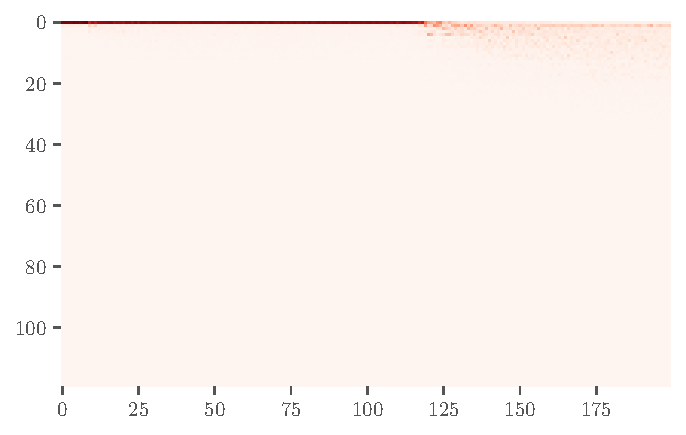
\includegraphics[width=\textwidth]{Figures/Correspondence/LeNet5_fixlr0.01/xxT_Trueest_real_corr_expand_t200_CIFAR10_Exp1_LeNet5_fixlr0.01R2_E-1_fc1.pdf}
%         \caption{$\mH$ with $\E[\vx\vx^\T]$}
%         \label{fig:Corr_xxT_True_fc}
%     \end{subfigure}%
%     \begin{subfigure}[t]{0.23\textwidth}
%         \centering
%         \captionsetup{justification=centering}
%         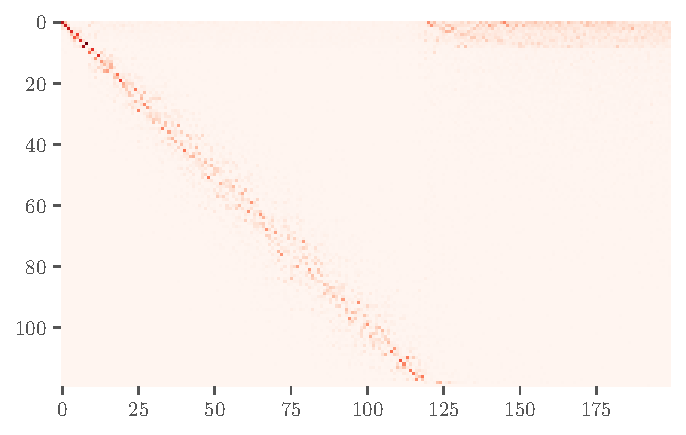
\includegraphics[width=\textwidth]{Figures/Correspondence/LeNet5_fixlr0.01/UTAU_Trueest_real_corr_expand_t200_CIFAR10_Exp1_LeNet5_fixlr0.01R2_E-1_fc1.pdf}
%         \caption{$\mH$ with $\E[\mM]$}
%         \label{fig:Corr_UTAU_True_fc}
%     \end{subfigure}%
%     \begin{subfigure}[t]{0.23\textwidth}
%         \centering
%         \captionsetup{justification=centering}
%         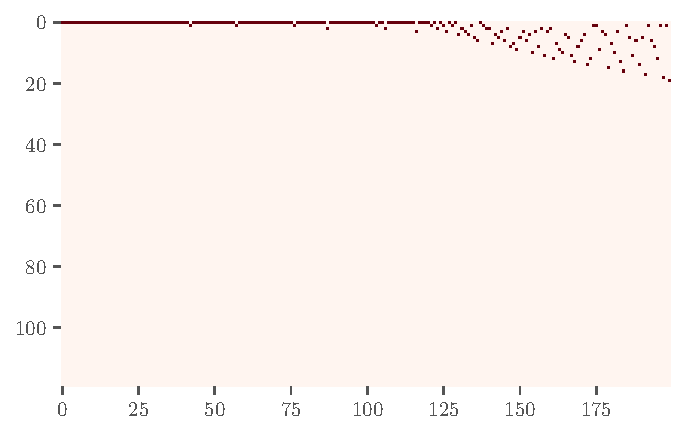
\includegraphics[width=\textwidth]{Figures/Correspondence/LeNet5_fixlr0.01/xxT_Approxest_real_corr_expand_t200_CIFAR10_Exp1_LeNet5_fixlr0.01R2_E-1_fc1.pdf}
%         \caption{$\hat{\mH}$ with $\E[\vx\vx^\T]$}
%         \label{fig:Corr_xxT_Approx_fc}
%     \end{subfigure}%
%     \begin{subfigure}[t]{0.23\textwidth}
%         \centering
%         \captionsetup{justification=centering}
%         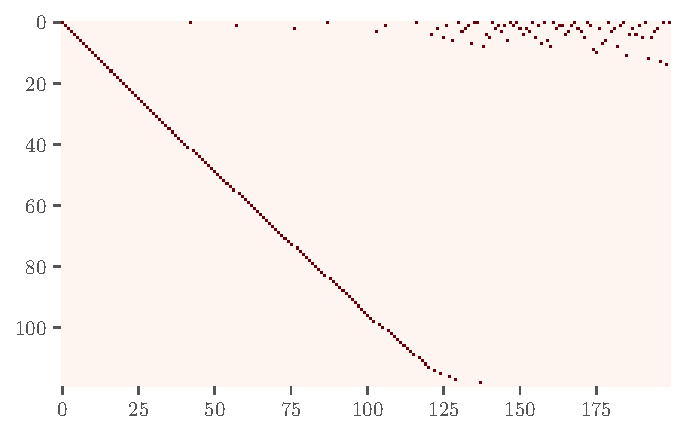
\includegraphics[width=\textwidth]{Figures/Correspondence/LeNet5_fixlr0.01/UTAU_Approxest_real_corr_expand_t200_CIFAR10_Exp1_LeNet5_fixlr0.01R2_E-1_fc1.pdf}
%         \caption{$\hat{\mH}$ with $\E[\vx\vx^\T]$}
%         \label{fig:Corr_UTAU_Approx_fc}
%     \end{subfigure}%
%     \begin{subfigure}[t]{0.032\textwidth}
%         \centering
%         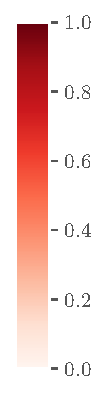
\includegraphics[width=\textwidth]{Figures/Misc/colorbar.pdf}
%     \end{subfigure}
%     }
%     %\captionsetup{justification=centering}
%     \caption{Heatmap of Eigenvector Correspondence Matrices for fc1:LeNet5, which has 120 output neurons. Here we take the top left corner of the eigenvector correspondence matrices. Similarities between (a)(c) and (b)(d) respectively verify the decoupling conjecture.}
%     \vspace{-0.1in}
%     \label{fig:Corr_fc}
% \end{figure*}

% In \figureref{fig:Corr_fc} we can see that the correspondence matrices for the true layer-wise Hessian $\mH$ approximately satisfies this property for top eigenvectors. The similarity between the correspondence patterns for the true and Kroneckor product approximated Hessian $\hat{\mH}$ also verifies the validity of the Kronecker approximation for dominate eigenspace.
% %Also note that since we are using Kronecker product to construct the approximated Hessian, the correspondence matrices of the approximated Hessian should have the ``perfect correlation''.
% From \figureref{fig:Corr_xxT_True_fc} and \figureref{fig:Corr_xxT_Approx_fc}, the top $m$ eigenvectors of the true layer-wise Hessian and the approximated Hessian are all highly correlated with $\vv_1$, the first eigenvector of $\E[\vx\vx^\T]$. From \figureref{fig:Corr_UTAU_True_fc} and \figureref{fig:Corr_UTAU_Approx_fc}, the correspondence with the $\E[\mM]$ component has a near diagonal pattern for both the true Hessian and the Kronecker approximation. Thus for small $i$ we have $\vh_i\approx \vv_1\otimes \vu_i$.
% %\rnote{Rong stopped here.}



% To understand the structure of $\E[\mM]$ itself, we consider a simplified setting where we have a random two-layer neural network with random data.
% \begin{theorem}[informal]
% For a two-layer neural network with Gaussian input, at initialization, when the network is large, the output Hessian of the first layer is approximately rank $(c-1)$ and the corresponding top eigenspace is $\gR(\mW^{(2)})\backslash\{\mW^{(2)}\cdot\textbf{1}\}$ and $\gR(\mW^{(2)})$ denotes the row space of the weight matrix $\mW^{(2)}$ of the second layer.
% \label{thm:gaussian_low_rank}
% \end{theorem}
% % To prove this theorem, we show that even after conditioning on $\mW$, the output of the network is approximately Gaussian, and is also weakly independent with the activations. These observations allows us to have a closed-form for the Hessian matrix and we leverage its form to prove the low rank structures. Note that even though the phenomenon that outputs are approximately Hessian is similar to recent works which understands wide networks as Gaussian processes \citep{lee2017deep}, the proof techniques are very different as we need to condition on $\mW$ while the Gaussian process critically relies on the fact that $\mW$ is random.

% The formal statement of this theorem and the full proof is in \sectionref{sec:appendix_low_rank}.
% The closed form calculation can be heuristically extended to the case with multiple layers, that the top eigenspace of the output Hessian of the $k$-layer would be approximately $\gR(\mS^{(k)})\setminus\{\mS^{(k)}\cdot\textbf{1}\}$,
% %$\gR\left(\mS^{(k)}\right)\setminus\{\mS^{(k)}\cdot\textbf{1}\}$, 
% %\begin{equation}
% %    \label{eqn:M-approx}
% %    \gR(\mS^{(k)})\setminus\{\mS^{(k)}\cdot\textbf{1}\}
% %\end{equation}
% where $\mS^{(k)} = \mW^{(n)}\mW^{(n-1)}\cdots\mW^{(k+1)}$ and $\gR(\mS^{(k)})$ is the row space of $\mS^{(k)}$.

% Though our result was only proven for random initialization and random data, we observe that this subspace also has high overlap with the top eigenspace of output Hessian at the minima of models trained with real datasets. The corresponding empirical results are shown in \sectionref{sec:app_outhessian_exp}. %\znote{Random Label not sufficiently discussed here: The estimation is indeed worse, which actually fits with \figureref{fig:UTAU_H_spec_RL}}
% % \begin{table}[H]
% % \vskip -0.15in
% % \caption{Overlap of $ \gR(\mS^{(k)})\setminus\{\mS^{(k)}\cdot\textbf{1}\}$ and the top $c-1$ dimension eigenspace of $\E[\mM^{(k)}]$ of different layers at minima.}
% % \vskip 0.1in
% % \begin{center}
% % \begin{small}
% % % \begin{sc}
% % \begin{tabular}{ccccccccc}
% % \toprule
% % Dataset & \multicolumn{2}{c}{MNIST} & \multicolumn{2}{c}{MNIST-R} & \multicolumn{2}{c}{CIFAR10} & \multicolumn{2}{c}{CIFAR10-R} \\
% % Network & F-$1500^3$    & LeNet5    & F-$1500^3$     & LeNet5     & F-$1500^3$     & LeNet5     & F-$1500^3$      & LeNet5     \\ \midrule
% % fc1     & 0.602         & 0.890     & 0.235          & 0.518      & 0.880          & 0.951      & 0.903           & 0.213       \\
% % fc2     & 0.967         & 0.931     & 0.801          & 0.912      & 0.943          & 0.972      & 0.931           & 0.701       \\
% % fc3     & 0.982         & 0.999     & 0.998          & 0.999      & 0.993          & 0.999      & 0.996           & 0.999     \\ \bottomrule
% % \end{tabular}
% % % \end{sc}
% % \end{small}
% % \end{center}
% % \label{tab:approx-m}
% % \vskip -0.15in
% % \end{table}
% % % \znote{This table can be compressed}
% % Note that the overlap can be low for random-label datasets which do not have a clear eigengap (as in \figureref{fig:UTAU_H_spec}). Understanding how the data could change the behavior of the Hessian is an interesting open problem. Other papers have given alternative explanations which are not directly comparable to ours, however ours is the only one that gives a closed-form formula for top eigenspace. In \sectionref{sec:appendix_M_struct} we will discuss the other explanations in more details.

% %We investigate why outliers occur in \sectionref{sec:appendix_M_struct} and explained the case at initialization.
% %Other paper has different explanations. For example,
% %\citet{papyan2019measurements} provides explanation for the low rank structure of hessian at minima using class clustering. However, in the setting of \cref{thm:gaussian_low_rank} such a clustering cannot happen because labels are also random. Our results are therefore incomparable. We discuss this in more detail in \sectionref{sec:appendix_M_struct}. \znote{The papyan paper explains the outliers at the minima using class clustering, Thm 4.1 was on initialization.}
% %\ynote{Should we mention we try to explain the outliers in the Appendix? Actually only the outlier for initialization is explained. We can say "We investigate the relation between structure of E[M] and outliers shown in Appendix" or "We explain the outliers at initialization in the Appendix"}
% %While previous work \citet{papyan2019measurements} provided some explanations for the gap using a clustering effect, such clustering does not happen in all of our experiments (and especially weak when the network is trained with random labels). 

% %\citet{papyan2019measurements} provides explanation for the gap in eigenspectrum using class clustering. Although we reproduced their results on their networks, there is no clear class clustering for both $\E[M]$ and layer-wise Hessian at the Minimum for networks we experiment on. The reason is unclear but we conjecture that class clustering is only significant for very large networks.

% %The outliers at initialization, however, are easier to explain. Similar to what \citet{papyan2019measurements} suggested for full Hessian, we observe logit clustering in $\E[\mM]$'s. Since there are $C$ logits, we would expect there are $C$ outliers. The results are shown in Appendix.